\chapter{Estimation Results and Discussions}
\label{ch: Results}

Initially, the estimation software was applied to the original mathematical model (equation \ref{eq: summary_original}) presented in Section \ref{sec: WPP_model}, developed to represent wind power plants. The hybrid estimation method presented in Section \ref{sec: Hybrid_Method} was applied, with MVMO providing a smart initial solution that will be refined by TSM. The results of the estimation process are shown in the following section of this chapter. In addition, studies on the effects of population size on MVMO convergence time were also conducted and its results are presented. In the end, the application of the estimation software to the proposed mathematical model (equation \ref{eq: summary_proposed}) is also presented in this chapter.

Besides, in order to evaluate the package support on different electrical equipment models, it was used to estimate the parameters of a Linearized Z-IM Load Model. The estimation of this model is presented in the appendix \ref{ch: appendix}.

\section{Parameter Estimation of Original WPP Model}

The original model equation \eqref{eq: summary_original} developed in Section \ref{sec: WPP_model} was used in this case. The estimation was conducted using the disturbance data collected in \cite{Cari2015} as the real system output. In such study, a fault was simulated on a test system using \textit{PowerFactory 14} and the data was used to estimate the parameters of the WPP model using only TSM. The system was simulated during $1\ s$ with measurements taken every $0.001\ s$. The fault was applied at $t=0.1\ s$ and was cleared out by the protection devices at $t=0.3\ s$. Figure \ref{fig: test_system} displays the test system used to collect data and Figure \ref{fig: WPP_voltage} depicts the WPP bus voltage measured during simulation.

\begin{figure}[!h]
	\caption{Test system simulated}
	\begin{center}
		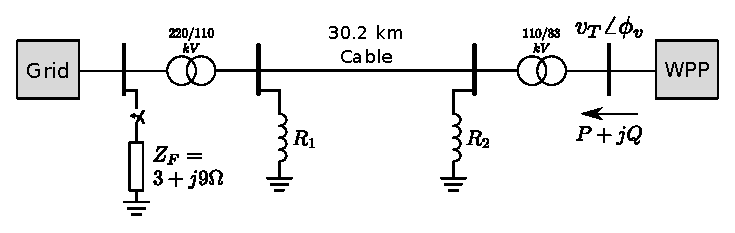
\includegraphics[scale=1]{Images/Cari_test_system.eps}
	\end{center}
	\label{fig: test_system}
\end{figure}

\begin{figure}[!h]
	\centering
	\caption{WPP bus voltage}
	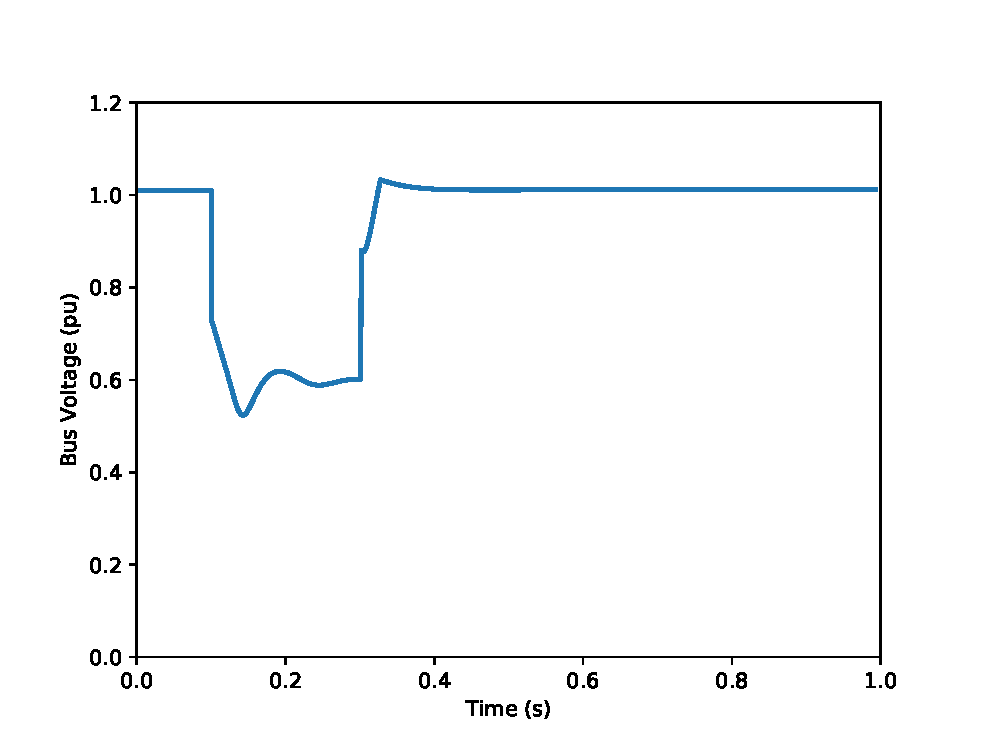
\includegraphics[scale=.7]{Images/bus_voltage.eps}
	\label{fig: WPP_voltage}
\end{figure}

MVMO search region was defined as depicted in Table \ref{tab: MVMO_boundaries}. These boundaries were decided based on the values previously found in \cite{Cari2015}.

\begin{table}[!h]
	\centering
	\caption{MVMO search region}
	\begin{tabular}{c|cc}
		Parameter & \shortstack{Lower \\ boundary} & \shortstack{Upper \\ boundary} \\\hline
		R & 0.027 & 0.040 \\
		X & 0.16 & 0.24 \\
		$k_{I}$ & 5.58 & 8.37 \\
		$T_{I}$ & 0.028 & 0.043 \\
		$T_{V}$ & 0.22 & 0.32 \\
		$k_{VC}$ & 1.60 & 2.40 \\
		$i_{max}$ & 0.88 & 1.32
	\end{tabular}
	\label{tab: MVMO_boundaries}
\end{table}

At first, 15 individuals (set of parameters) were randomly generated inside this given region, evaluated and ranked according to their error $J(p)$. At every generation, three parameters of the fittest individual would suffer mutation in order to generate a new individual. This process continued until the fittest individual reached an error level below a tolerance of $tol_{1} = 0.5$. If this criterion were not met, MVMO would halt when the \nth{5000} generation was reached.

The fittest individual found by MVMO was then used as the starting point to TSM. Since this method converges quickly when close to the optimal solution, it was configured to run for only 7 iterations. Its goal was to find a set of parameters with $J(p)$ below $tol_{2} = 5\times10^{-4}$.

The parameters were estimated in 8.11 seconds in total, with MVMO and TSM taking 4.19 and 3.92 seconds, respectively, resulting in an error $J(p)$ of $1.5\times 10^{-4}$. The value estimated for each parameter is displayed in the Table \ref{tab: results}.

\begin{table}[h]
	\centering
	\caption{Estimated values of parameters}
	\begin{tabular}{c|c}
		Parameter & \shortstack{Estimated \\ value} \\\hline
		R & 0.034 \\
		X & 0.198 \\
		$k_{I}$ & 6.333 \\
		$T_{I}$ & 0.0348 \\
		$T_{V}$ & 0.246 \\
		$k_{VC}$ & 1.999 \\
		$i_{max}$ & 1.100
	\end{tabular}
	\label{tab: results}
\end{table}

Figures \ref{fig: output_P} and \ref{fig: output_Q} depict, respectively, real and active power measured from the simulated system and calculated using the WPP model with estimated parameters. For both components, the model output matches almost exactly with the curve expected. Therefore, the WPP model adjusted with the parameter vector found is able to reproduce the behaviour of the same wind power plant in similar conditions.

\begin{figure}[h]
	\centering
	\caption{Active power of real system (measured) and mathematical model (simulated) after parameter estimation}
	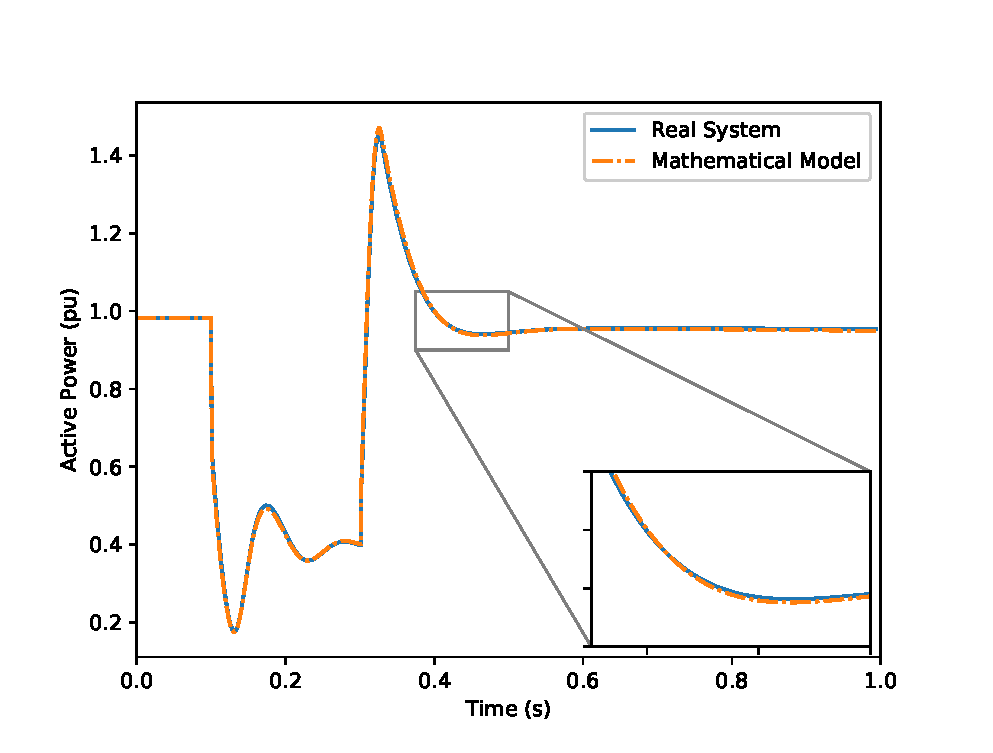
\includegraphics[scale=0.7]{Images/P_compared.eps}
	\label{fig: output_P}
\end{figure}

\begin{figure}[h]
	\centering
	\caption{Reactive power of real system (measured) and mathematical model (simulated) after parameter estimation}
	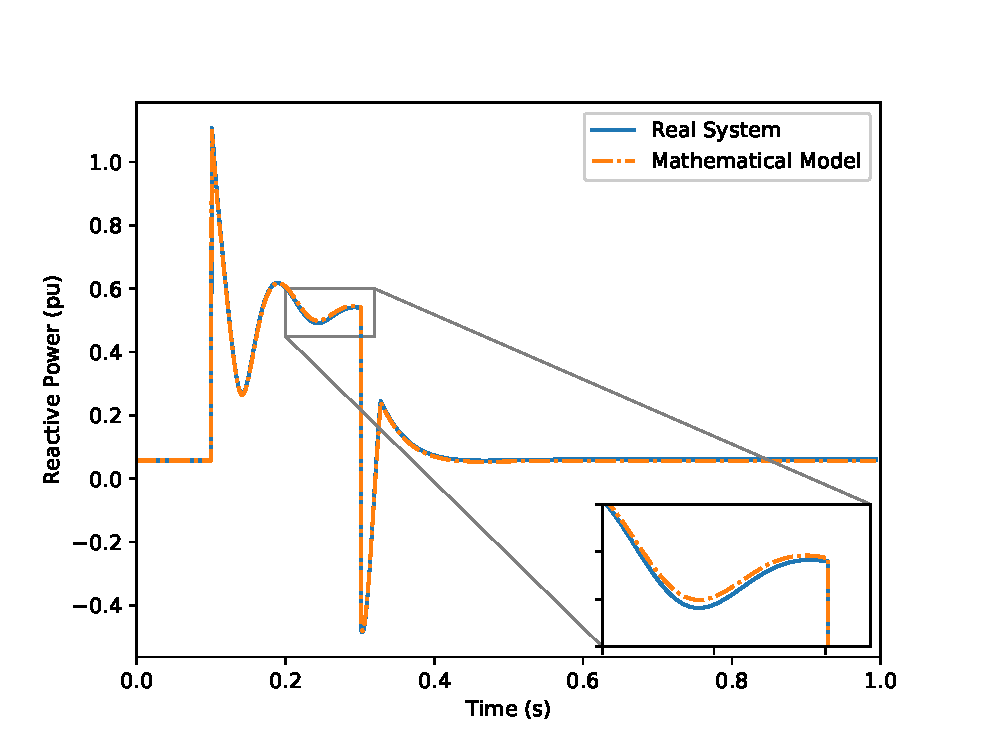
\includegraphics[scale=0.7]{Images/Q_compared.eps}
	\label{fig: output_Q}
\end{figure}

\subsection{Influence of MVMO Population Size}

In order to evaluate how the population size affects MVMO, a series of estimations using only this method were executed varying only the number of individuals. Five population sizes were chosen for this experiment (5, 10, 20, 50 and 100 individuals) and, for each one of them, 35 estimations were executed.

Apart from population size, all method configurations were fixed, so the results could be directly compared. The error tolerance was set at $tol_{1} = 0.5$ and the search region was the same as presented in Table \ref{tab: MVMO_boundaries}. The mean duration of estimation for each population size is shown below.

\begin{table}[h]
	\centering
	\caption{Influence of population size in MVMO}
	\begin{tabular}{c|c}
		\shortstack{\# of \\ individuals} & \shortstack{Average \\ duration (s)} \\\hline
		5 & 15.62 \\
		10 & 11.08 \\
		20 & 13.02 \\
		50 & 17.84 \\
		100 & 29.00 
	\end{tabular}
	\label{tab: pop_size}
\end{table}

For considerably small populations (less than 5 individuals), the algorithm has to further explore the search region, due to reduced number of candidates. On the other extreme, large populations (more than 50 individuals) usually present good candidates in their initial population, only requiring a refinement of the solution. However, generating and evaluating all initial candidates has a huge cost, impacting on the estimation time. For these reasons, populations of 10 to 20 individuals present better convergence times than others, as depicted in Table \ref{tab: pop_size}.

\section{Parameter Estimation of Proposed WPP Model}

The proposed model equation \eqref{eq: summary_proposed} developed in Section \ref{sec: WPP_model} was used in this case. Given the similarities between original and proposed models, the simulations of the latter were conducted using the same parameter values found for the former. It was observed that, in order to adjust the pre-fault behaviour of the proposed model, the upper limit of the delay blocks should be increased to at least $V_{max} = 1.1$. With these changes made, the outputs of the proposed model (with the parameters presented in Table \ref{tab: results}) were compared to the original WPP model, as displayed in Figures \ref{fig: proposed_P} and \ref{fig: proposed_Q}.

\begin{figure}[!h]
	\centering
	\caption{Active power from original and proposed models}
	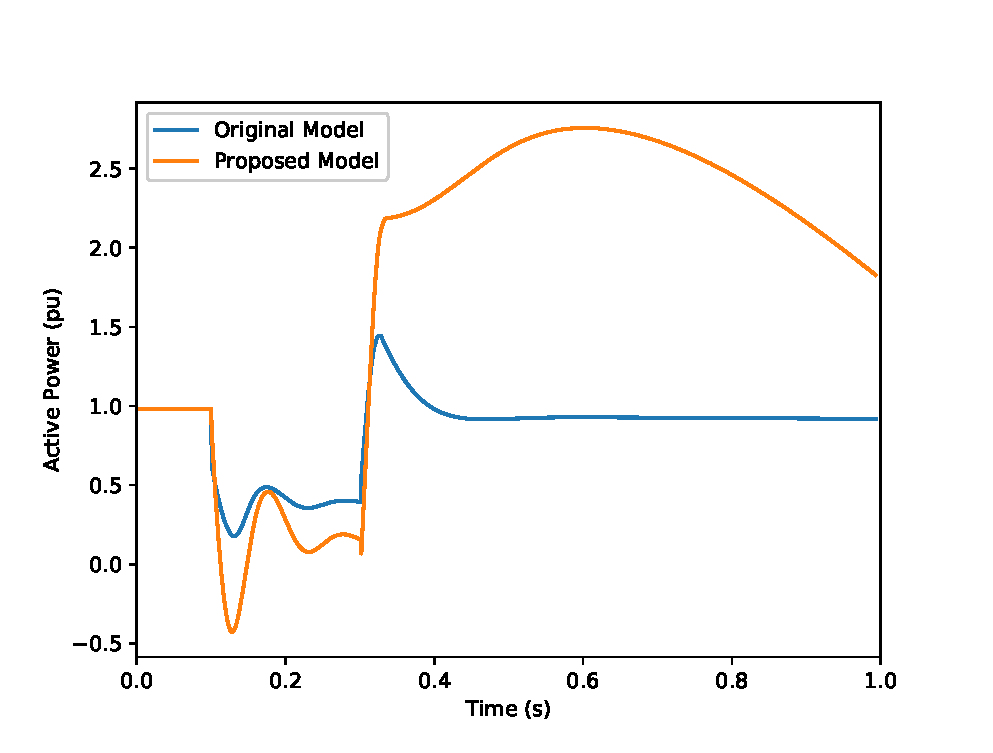
\includegraphics[scale=.7]{Images/P_proposed.eps}
	\label{fig: proposed_P}
\end{figure}

\begin{figure}[!h]
	\centering
	\caption{Reactive power from original and proposed models}
	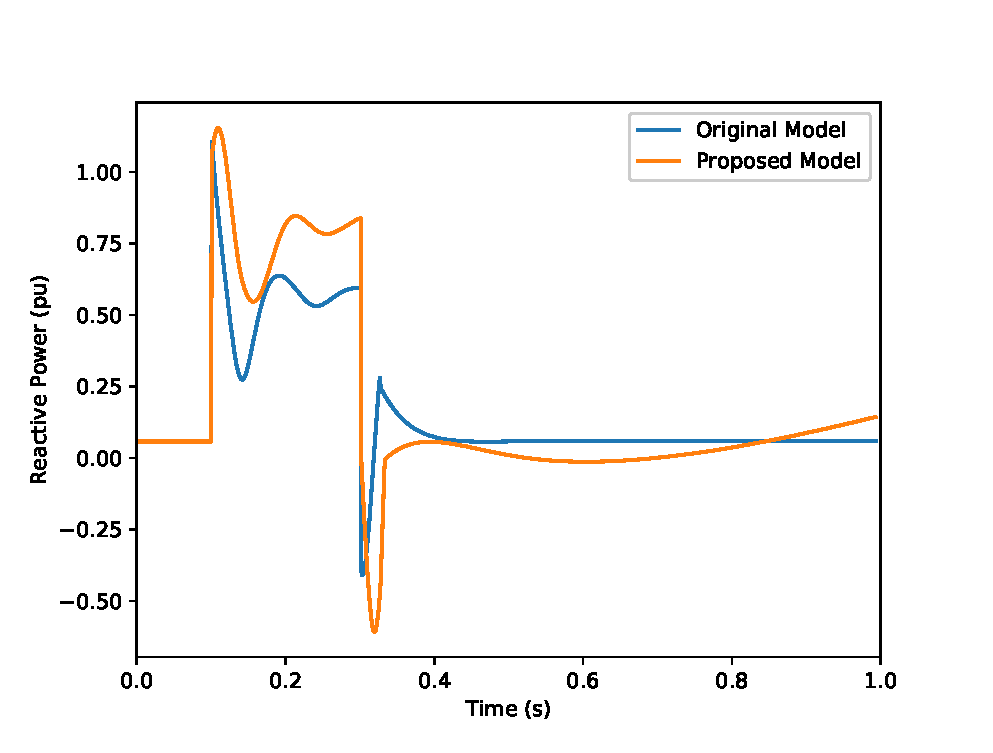
\includegraphics[scale=.7]{Images/Q_proposed.eps}
	\label{fig: proposed_Q}
\end{figure}

It can be noticed that reactive power obtained with the proposed model is not distant from the behaviour obtained with the original WPP model. Active power, on the other hand, diverged from the expected, specially during post-fault period. 

Afterwards, the hybrid estimation approach was applied in order to estimate the parameters of the proposed model. The configurations of the estimation conducted were the same as presented previously, with $tol_{1} = 0.5$ and $tol_{2}=5\times 10^{-4}$ and MVMO search region given by the boundaries presented in Table \ref{tab: MVMO_boundaries}. The parameters estimated are depicted in Table \ref{tab: results_proposed} and the behaviours of active and reactive power for this model are shown in Figures \ref{fig: estimation_proposed_P} and \ref{fig: estimation_proposed_Q}, respectively.

\begin{table}[h]
	\centering
	\caption{Estimated parameters for proposed model}
	\begin{tabular}{c|c}
		Parameter & \shortstack{Estimated \\ value} \\\hline
		R & 0.058 \\
		X & 0.499 \\
		$k_{I}$ & $4.3\times 10^{8}$ \\
		$T_{I}$ & 101.6 \\
		$T_{V}$ & $1.5\times 10^{7}$ \\
		$k_{VC}$ & 2.017 \\
		$i_{max}$ & 1.083 \\
		$V_{max}$ & 1.1
	\end{tabular}
	\label{}
\end{table}

\begin{figure}[!h]
	\centering
	\caption{Active power of proposed model after estimation}
	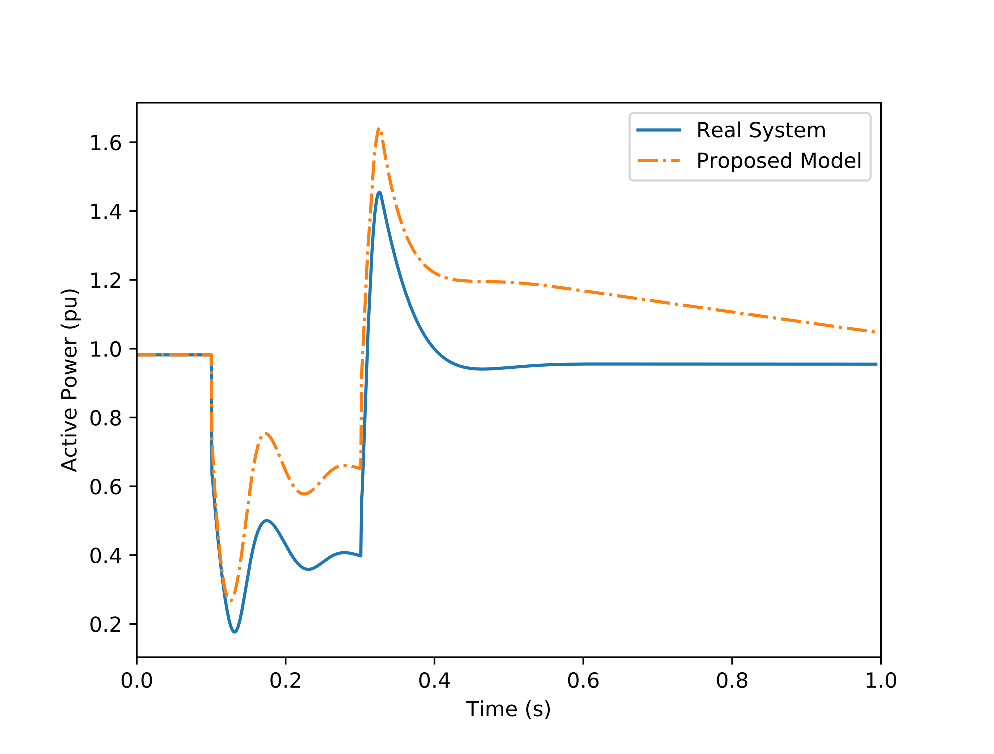
\includegraphics[scale=.7]{Images/P_proposed_estimated.eps}
	\label{fig: estimation_proposed_P}
\end{figure}

\begin{figure}[!h]
	\centering
	\caption{Reactive power of proposed model after estimation}
	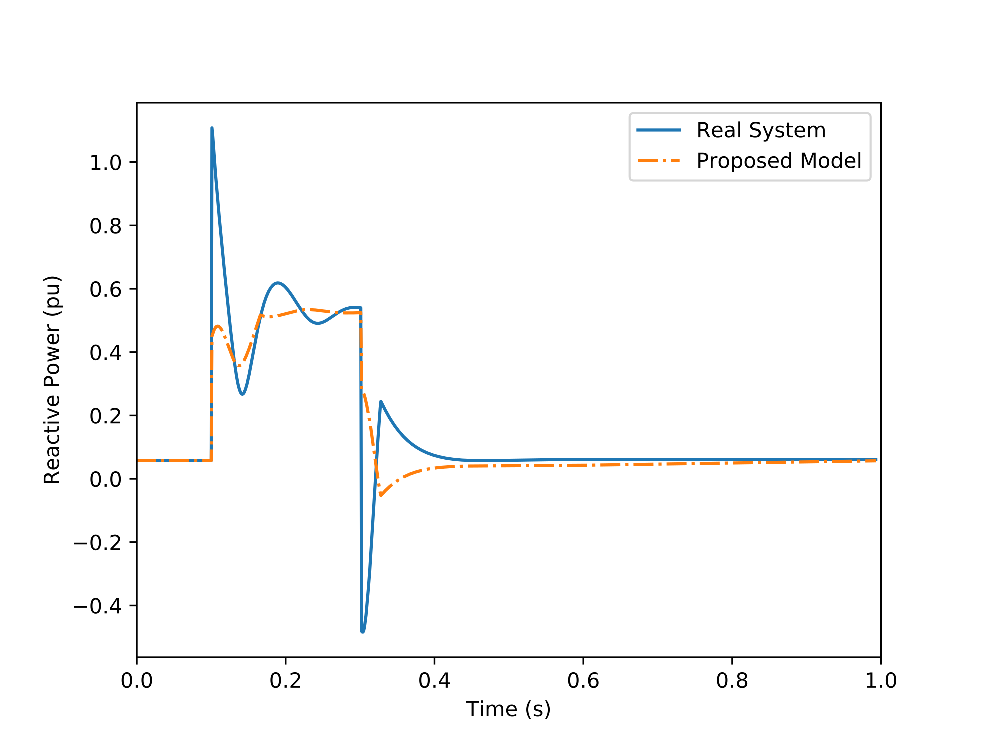
\includegraphics[scale=.7]{Images/Q_proposed_estimated.eps}
	\label{fig: estimation_proposed_Q}
\end{figure}

Despite the similarities between the behaviours of the proposed WPP model and the real system, the resulting parameter vector is not feasible, with extremely large values for some of the parameters, as shown in Table \ref{tab: results_proposed}. These results indicate that the proposed WPP model is not entirely able to represent wind power plants yet, requiring further studies for improvement.